\chapter{Introdução}

\section{Contextualização e Motivação}
%
O crescente interesse na exploração subaquática tem realçado a relevância dos manipuladores integrados a veículos autônomos, formando os chamados Sistemas Manipuladores-Veículos Subaquáticos (UVMSs). Segundo Antonelli \cite{antonelli2014modelling}, esses sistemas permitem a execução autônoma de tarefas complexas em ambientes inóspitos, superando os altos custos, riscos e limitações associados à operação humana direta. 

Além de seu valor estratégico em operações \textit{offshore} e científicas, os UVMSs oferecem uma oportunidade única do ponto de vista da engenharia, o qual é a sua redundância cinemática que pode ser explorada para otimização energética e aumento de manipulabilidade.

No entanto, o estudo e o desenvolvimento de controladores para esses sistemas enfrentam barreiras substanciais. A primeira é a natureza física do ambiente: conforme Aldhaheri et al. \cite{aldhaheri2022underwater}, a imprevisibilidade do meio marinho e as forças hidrodinâmicas acopladas dificultam a plena autonomia.

A segunda barreira, frequentemente subestimada, é o desafio computacional e educacional da modelagem. A dinâmica de um UVMS é regida por equações diferenciais não-lineares de alta complexidade. Tradicionalmente, o ensino e a pesquisa nessa área dependem de softwares proprietários (como MATLAB/Simulink). Embora robustas, essas ferramentas atuam muitas vezes como ``caixas-pretas'', ocultando a formulação matemática explícita do aluno e impondo um gargalo computacional severo: a transição entre a modelagem simbólica (necessária para derivar as equações exatas) e a simulação numérica em tempo real é frequentemente lenta ou exige ferramentas de compilação complexas.

Dada a elevada complexidade necessária para modelar e simular um manipulador subaquático com múltiplos graus-de-liberdade, torna-se imperioso buscar abordagens acessíveis e computacionalmente eficientes.  

\section{Justificativa}
%
A motivação para o desenvolvimento deste trabalho surge da necessidade de democratizar o acesso a ferramentas de simulação de alta fidelidade e superar as limitações de integração observadas em ambientes clássicos de engenharia.

Historicamente, a dinâmica de sistemas multicorpos é ensinada de forma desconexa da implementação. Quando se busca precisão via toolboxes comerciais, esbarra-se no custo de licenças e na rigidez da arquitetura de software, o que dificulta a experimentação de novos algoritmos por estudantes e pesquisadores independentes. Esse gargalo de software é particularmente crítico na robótica marinha. Como afirmam Yuh e West \cite{yuh2001underwater}, a adição de manipuladores transforma o veículo em um sistema multicorpos de modelagem altamente complexa, tornando o uso de simulações precisas e integradas uma etapa obrigatória para lidar com os altos custos e riscos dos testes reais..

Neste contexto, a migração para o ecossistema Python apresenta-se como a solução técnica ideal, permitindo a integração de bibliotecas de computação simbólica (SymPy) com o ecossistema científico e numérico para um fluxo de trabalho contínuo \cite{meurer2017sympy}. Para contornar os gargalos de desempenho inerentes à manipulação simbólica pura \cite{meurer2017sympy}, a abordagem proposta neste trabalho utiliza as capacidades de geração de código do SymPy aliadas à Eliminação de Subexpressões Comuns (\textit{Common Subexpression Elimination}, CSE) \cite{meurer2017sympy}. Assim, através da compilação \textit{Just-in-Time} via \texttt{lambdify}, a modelagem lagrangiana do sistema é convertida diretamente em código de máquina vetorizado (NumPy) e otimizado para simulações de alta performance.

A concretização da ``plataforma didática'' passa ainda pela existência de uma interface gráfica (\textit{Graphical User Interface}, GUI) desenvolvida com a biblioteca CustomTkinter, que torna o ambiente acessível sem a necessidade de programação direta. Essa interface estrutura-se em três módulos funcionais: \textbf{Modelagem} (configuração da cadeia cinemática e geração simbólica do modelo dinâmico), \textbf{Simulação} (definição de trajetórias, controladores e parâmetros físicos) e \textbf{Análise} (comparação entre múltiplas sessões de controle).

Assim, este trabalho justifica-se pela criação do ambiente \textit{Hephaestus}: uma ferramenta que não apenas modela os efeitos hidrodinâmicos (massa adicionada, arrasto, empuxo) com rigor matemático, mas também serve como plataforma didática e \textit{open-source} para a validação de estratégias de controle avançado, unindo a teoria de Dinâmica e Controle à moderna Engenharia de Software. Sintetiza-se, na Figura~\ref{fig:arquitetura_geral}, a arquitetura geral do \textit{Hephaestus}, com destaque para o fluxo de trabalho que vai da especificação simbólica da cadeia cinemática até a comparação das estratégias de controle.

\begin{figure}[htbp]
    \centering
    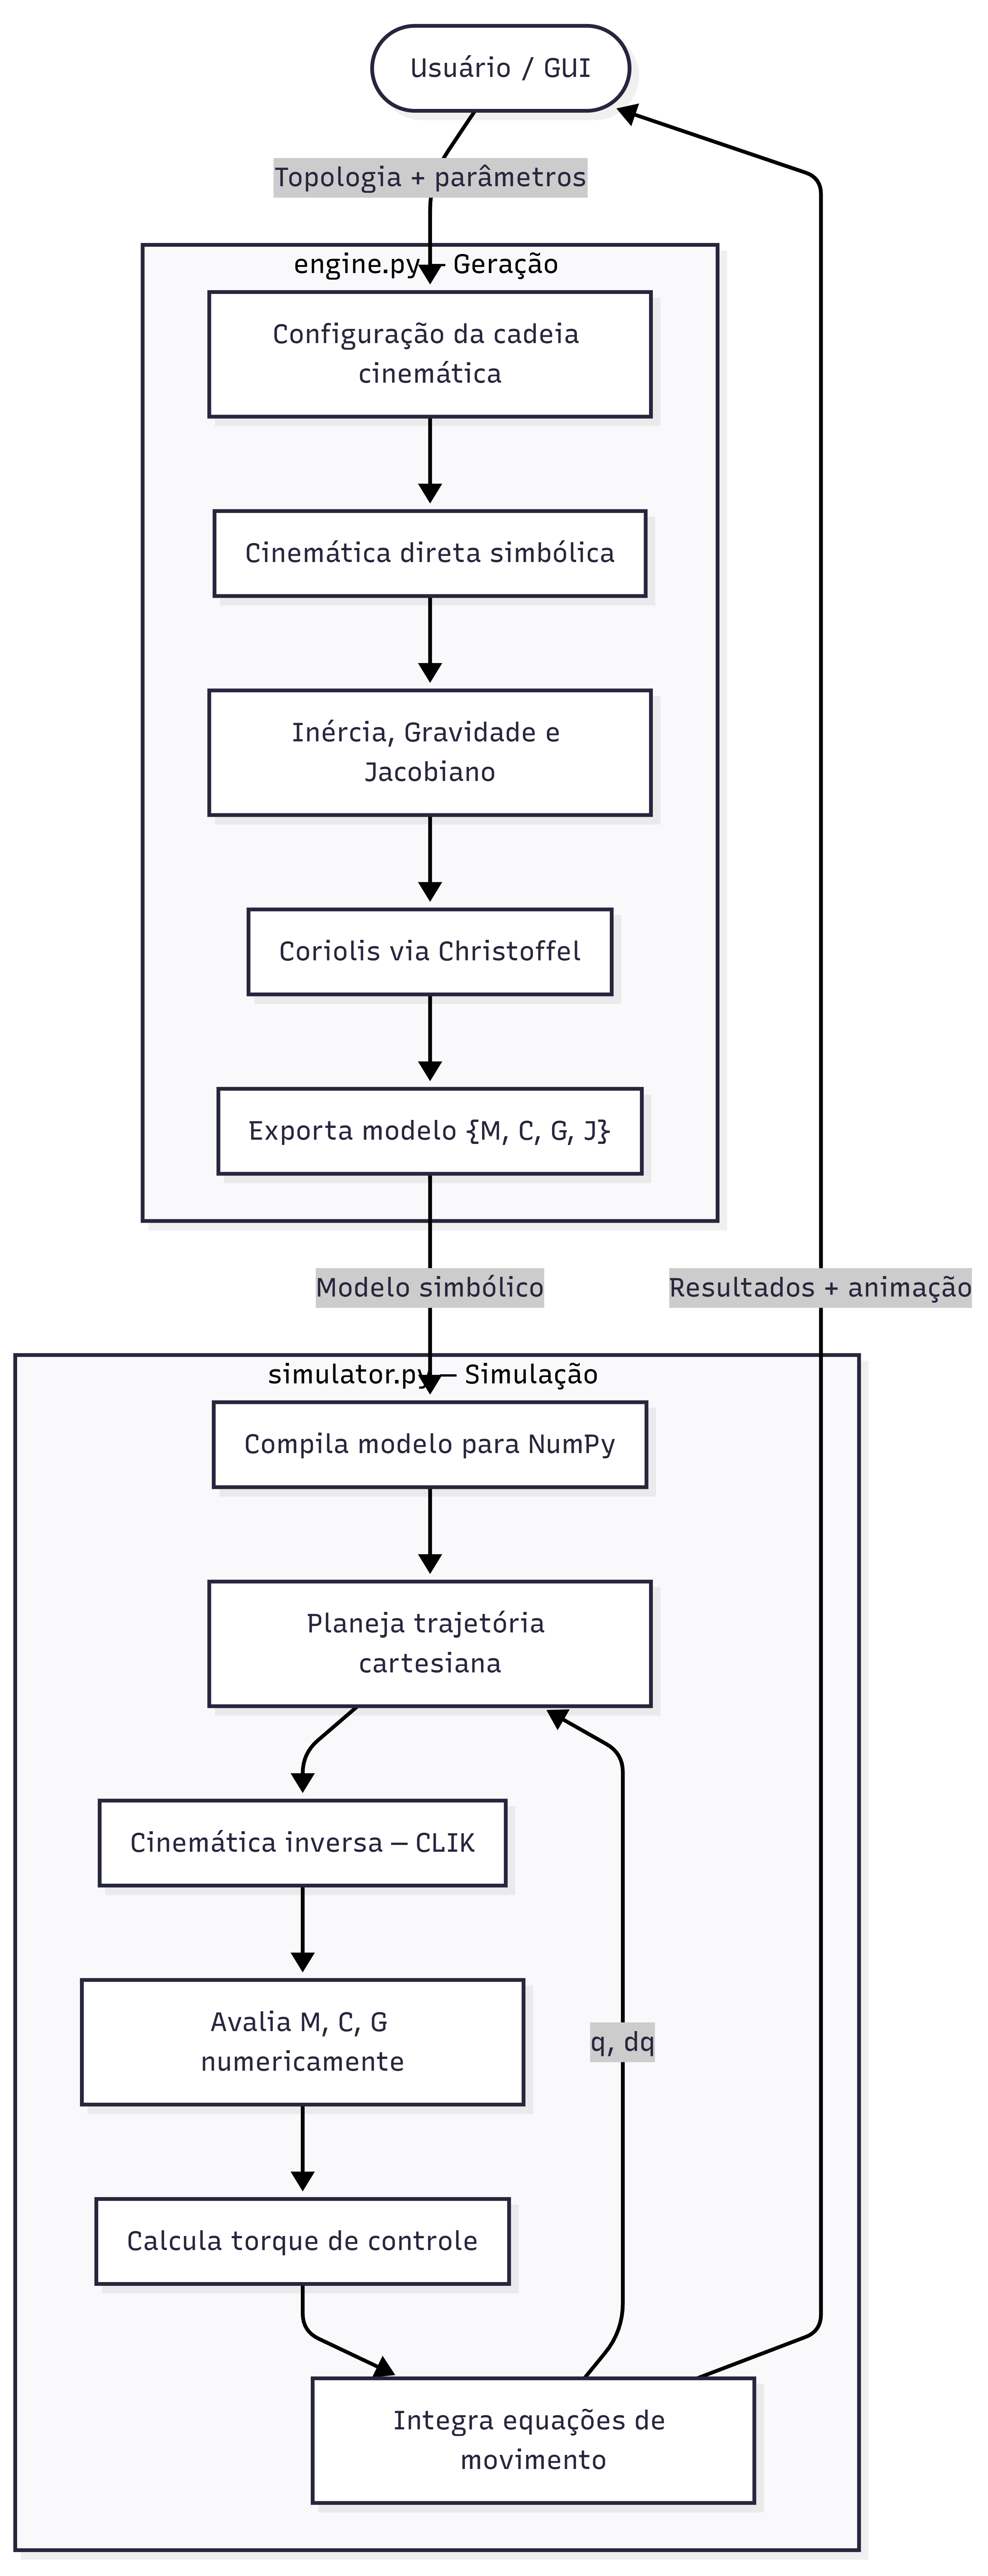
\includegraphics[width=0.50\textwidth]{figuras/Diagramas/Diagrama 1 — Arquitetura Geral do Sistema.png}
    \caption{Arquitetura geral do ambiente \textit{Hephaestus}: fluxo de trabalho desde a especificação da cadeia cinemática (módulo Modelagem) até a simulação em malha fechada (módulo Simulação) e a comparação de resultados (módulo Análise). As dependências entre os módulos \texttt{engine.py} e \texttt{simulator.py} e os quatro controladores não-lineares são destacadas.}
    \label{fig:arquitetura_geral}
\end{figure}

\section{Objetivos}

\subsection{Objetivo Geral}
Desenvolver um ambiente computacional integrado em Python para a modelagem dinâmica simbólica e simulação de manipuladores robóticos e sistemas UVMS. O projeto visa implementar uma arquitetura que automatize a derivação das equações de movimento via formulação Lagrangiana e execute simulações de controle em malha fechada com alto desempenho, considerando explicitamente os efeitos hidrodinâmicos, o controle no \emph{espaço de tarefa 6D} (posição $+$ orientação) e a comparação entre múltiplas estratégias de controle não-linear.

\paragraph{O que é o espaço de tarefa 6D.}
O termo ``6D'' refere-se à descrição completa da \emph{pose} do efetuador no espaço cartesiano, dada por seis coordenadas independentes: três para a \textbf{posição} e três para a \textbf{orientação}. As três coordenadas de posição $(x, y, z)$ localizam um ponto de referência do efetuador no espaço, enquanto as três coordenadas de orientação , tipicamente representadas por ângulos de \textit{roll}, \textit{pitch} e \textit{yaw} ou, equivalentemente, pelo eixo-ângulo de uma rotação em $SO(3)$ , descrevem a sua atitude angular. Tarefas de robótica que envolvem alinhar uma ferramenta a uma superfície, soldar ao longo de uma trajetória ou inserir uma peça em um furo exigem o controle simultâneo dessas seis coordenadas, e não apenas das três posicionais. Por essa razão, o \textit{Hephaestus} estende o algoritmo de cinemática inversa em malha fechada (CLIK) para operar com o Jacobiano completo $J \in \mathbb{R}^{6 \times N}$ , Capítulo~\ref{cap:revisao} , que mapeia as $N$ velocidades de junta para as seis componentes da \textit{twist} cartesiana (três lineares + três angulares).

\subsection{Objetivos Específicos}
\label{sec:Objetivos}

A fim de atingir o objetivo geral, foram definidos os seguintes objetivos específicos:

\begin{itemize}
    \item \textbf{Revisão Bibliográfica e Metodológica:} Analisar as abordagens clássicas de modelagem (Craig, Spong) e as especificidades da hidrodinâmica de UVMS (Fossen, Antonelli), identificando as limitações das ferramentas de simulação atuais.

    \item \textbf{Desenvolvimento da \textit{Engine} Matemática:} Implementar algoritmos em Python capazes de gerar simbolicamente as matrizes de Inércia ($M$), o vetor de Coriolis e Centrípeto ($C$) e o vetor de Gravidade/Empuxo ($G$) para manipuladores genéricos de $N$ graus de liberdade, tanto em ambiente terrestre quanto subaquático. No cenário subaquático, a massa adicionada é modelada como um tensor diagonal $6 \times 6$ por elo (três componentes translacionais e três rotacionais), rotacionado para o referencial global, em conformidade com a formulação de Fossen \cite{fossen2011handbook}.

    \item \textbf{Otimização Computacional:} Desenvolver um método de compilação das equações simbólicas para funções numéricas otimizadas por meio do \texttt{lambdify} com Eliminação de Subexpressões Comuns (CSE), superando os gargalos de desempenho típicos de simulações simbólicas puras. Implementar dois níveis de paralelismo: (i) na \textit{fase de derivação} do modelo, paralelizando o cálculo de $\partial M/\partial q_k$ e das linhas do vetor $C$ entre múltiplos processos; e (ii) na \textit{fase de simulação}, por meio de um executor de processos persistente (\texttt{ProcessPoolExecutor}) que avalia $M$, $C$ e $G$ numericamente em paralelo a cada passo de integração, eliminando o custo de \textit{respawn} entre execuções.

    \item \textbf{Implementação do Simulador Numérico:} Construir um ambiente de simulação capaz de resolver a dinâmica direta e inversa, incluindo: planejamento de trajetórias (segmentos de reta e arcos circulares com polinômio cúbico de interpolação); modelos de atrito nas juntas (Coulomb + viscoso, suavizados por $\tanh$ para evitar descontinuidades); e modelos de arrasto hidrodinâmico no espaço de juntas (linear e quadrático). Incluir visualização gráfica animada dos resultados.

    \item \textbf{Controle de Orientação no Espaço de Tarefa 6D:} Estender o algoritmo de Cinemática Inversa em Malha Fechada (CLIK) para o espaço de tarefa completo de seis dimensões, em que as três primeiras correspondem à posição cartesiana $(x, y, z)$ do efetuador e as três últimas à sua orientação angular (\textit{roll}, \textit{pitch}, \textit{yaw}), utilizando o Jacobiano completo $J \in \mathbb{R}^{6 \times N}$. Implementar múltiplos modos de referência de orientação: \textit{Livre}, \textit{Fixa}, \textit{Tangente à Trajetória}, \textit{Apontar para o Alvo}, interpolação SLERP (\textit{Spherical Linear Interpolation}) \cite{shoemake1985animating} e \textit{Normal à Superfície}.

    \item \textbf{Projeto e Validação de Controle:} Implementar e comparar quatro estratégias de controle não-linear em malha fechada:
    \begin{enumerate}
        \item \textbf{Controle por Torque Computado com PID} (CTC-PID): linearização por realimentação com termo integral \cite{craig1989introduction}, acrescido de uma compensação \textit{anti-windup} para evitar a instabilidade frente à saturação dos atuadores \cite{ogata2010modern}
        \item \textbf{Controle por Modo Deslizante} (CT-SMC): superfície deslizante \cite{slotine1991applied} com camada limite suavizante ($\tanh$) \cite{burton1986continuous};
        \item \textbf{Super-Twisting SMC} (STA): algoritmo de modo deslizante de 2ª ordem com sinal de controle contínuo e convergência em tempo finito \cite{levant1993sliding, moreno2012strict};
        \item \textbf{Controle por Rejeição Ativa de Distúrbios} (LADRC): observador de estado estendido (ESO) descentralizado com estimação e cancelamento em malha fechada dos distúrbios residuais \cite{han2009pid}.
    \end{enumerate}
    Todos os controladores são alimentados pelo algoritmo de Cinemática Inversa em Malha Fechada (CLIK). O tratamento de singularidades é realizado pelo método de Mínimos Quadrados Amortecidos (DLS) , formulado originalmente como Inversa Robusta a Singularidades (SR-Inverse) \cite{nakamura1986inverse} ,, e a gestão de redundância é estruturada via projeção no Espaço Nulo \cite{chiaverini1997singularity}.
\end{itemize}

\section{Metodologia}

A metodologia adotada estrutura-se em uma abordagem incremental de desenvolvimento de software e validação matemática:

\subsection{Modelagem Matemática (A Camada \textit{Engine})} Utilizando a biblioteca SymPy , em particular o módulo \texttt{dynamicsymbols} da mecânica analítica, que fornece símbolos dependentes do tempo com diferenciação automática , será implementada a formulação de Euler-Lagrange. Diferente de abordagens numéricas de caixa-preta, o software deduzirá as equações literais. Para o cenário subaquático, serão incorporados os termos de energia potencial aparente (Peso - Empuxo) e energia cinética modificada (Massa Adicionada como tensor 6D por elo), conforme Fossen \cite{fossen2011handbook}. O vetor resultante $C(q, \dot{q})$ unifica os efeitos de Coriolis e centrípeto pela formulação dos símbolos de Christoffel de primeira espécie \cite{spong2020robot}.

\subsection{Transição Simbólico-Numérica e Otimização}
Esta etapa foca na eficiência computacional e na superação do gargalo de desempenho típico de álgebras simbólicas. As equações dinâmicas geradas serão compiladas via \texttt{lambdify} com CSE (\textit{Common Subexpression Elimination}) ativo, que identifica e fatoriza subexpressões repetidas na expressão simbólica antes da geração do código NumPy, reduzindo o tamanho do \textit{bytecode} compilado e acelerando a avaliação numérica \cite{meurer2017sympy}.

Para lidar com a complexidade computacional do termo de Coriolis em sistemas de múltiplos graus de liberdade, será implementado processamento paralelo em dois níveis distintos. No primeiro nível, a derivação simbólica de $\partial M/\partial q_k$ e o cálculo das linhas do vetor $C$ são distribuídos entre múltiplos processos via \texttt{ProcessPoolExecutor}, visando otimizar o tempo de geração do modelo conforme as métricas de eficiência discutidas por Hollerbach \cite{hollerbach1980recursive}. No segundo nível, durante a simulação, um executor de processos persistente , pré-inicializado após a compilação e reutilizado em todos os ciclos subsequentes , avalia $M(q)$, $C(q, \dot{q})$ e $G(q)$ em paralelo a cada passo de integração, eliminando o custo de instanciação repetida de \textit{workers}.

\subsection{Simulação e Controle (A Camada \textit{Simulator}) }
\label{sec:simulador}
Será desenvolvido um integrador numérico Simplético de Euler operando em malha fechada. A escolha pelo método Simplético (atualização de $q$ antes de $\dot{q}$) em detrimento do Euler Explícito padrão é motivada pela melhor preservação da energia do sistema ao longo da trajetória. O passo de integração física pode ser subdividido (\textit{substeps}) de forma independente do passo de visualização, permitindo alta fidelidade numérica sem custo proporcional de renderização.

O controle dinâmico será realizado por uma das quatro estratégias implementadas (CTC-PID, CT-SMC, STA ou LADRC), todas alimentadas por um algoritmo de Cinemática Inversa em Malha Fechada (CLIK). A fase de inicialização da postura utiliza um algoritmo de Levenberg-Marquardt com busca em linha adaptativa, que ajusta dinamicamente o parâmetro de amortecimento $\lambda$ para garantir convergência robusta antes do início da trajetória. Durante a simulação, o CLIK opera no espaço de tarefa 6D (posição + orientação), incorporando: referência de velocidade e aceleração por \textit{feedforward}, correção de deriva do Jacobiano ($\dot{J}\dot{q}$), tratamento de singularidades via DLS \cite{nakamura1986inverse} e gestão de redundância via projeção no Espaço Nulo \cite{chiaverini1997singularity}.

Modelos de atrito nas juntas (Coulomb + viscoso, suavizados por $\tanh$) e de arrasto hidrodinâmico no espaço de juntas (linear e quadrático) são aplicados na equação de integração como forças passivas, separadamente do sinal de controle.

\subsection{Validação Comparativa}
O software desenvolvido (\textit{Hephaestus}) será submetido a testes de trajetória em dois cenários distintos: um manipulador serial em ambiente terrestre e um UVMS em ambiente submerso. A validação do cenário submerso seguirá os critérios de modelagem hidrodinâmica estabelecidos por Fossen e Antonelli \cite{fossen2011handbook, antonelli2014modelling}, analisando comparativamente os torques requeridos, o erro de rastreamento de posição e orientação, e o comportamento frente a perturbações externas para confirmar a consistência física dos termos de massa adicionada e empuxo implementados. A comparação entre as quatro estratégias de controle será realizada na aba de \textbf{Análise} da interface gráfica, que permite sobrepor múltiplas sessões de simulação nos mesmos gráficos.
